\newcommand*{\ClipSep}{0.5cm}
\def\face#1{
\begin{tikzpicture}
\node [inner sep=0pt] at (0,0) {\includegraphics[width=3.0cm]{#1}};
\draw [white, rounded corners=\ClipSep, line width=\ClipSep] 
    (current bounding box.north west) -- 
    (current bounding box.north east) --
    (current bounding box.south east) --
    (current bounding box.south west) -- cycle
    ;
\end{tikzpicture}
}


%
% Committee
%
\begin{frame}{Thanks!}
\begin{center}
\face{../img/chris.jpg}
\face{../img/percy.jpg}
\face{../img/dan.jpg}
\\
\face{../img/potts.jpg}
\face{../img/tom.jpg}
\end{center}
\end{frame}


%
% Family
%
\begin{frame}[noframenumbering]{Thanks!}
\begin{center}
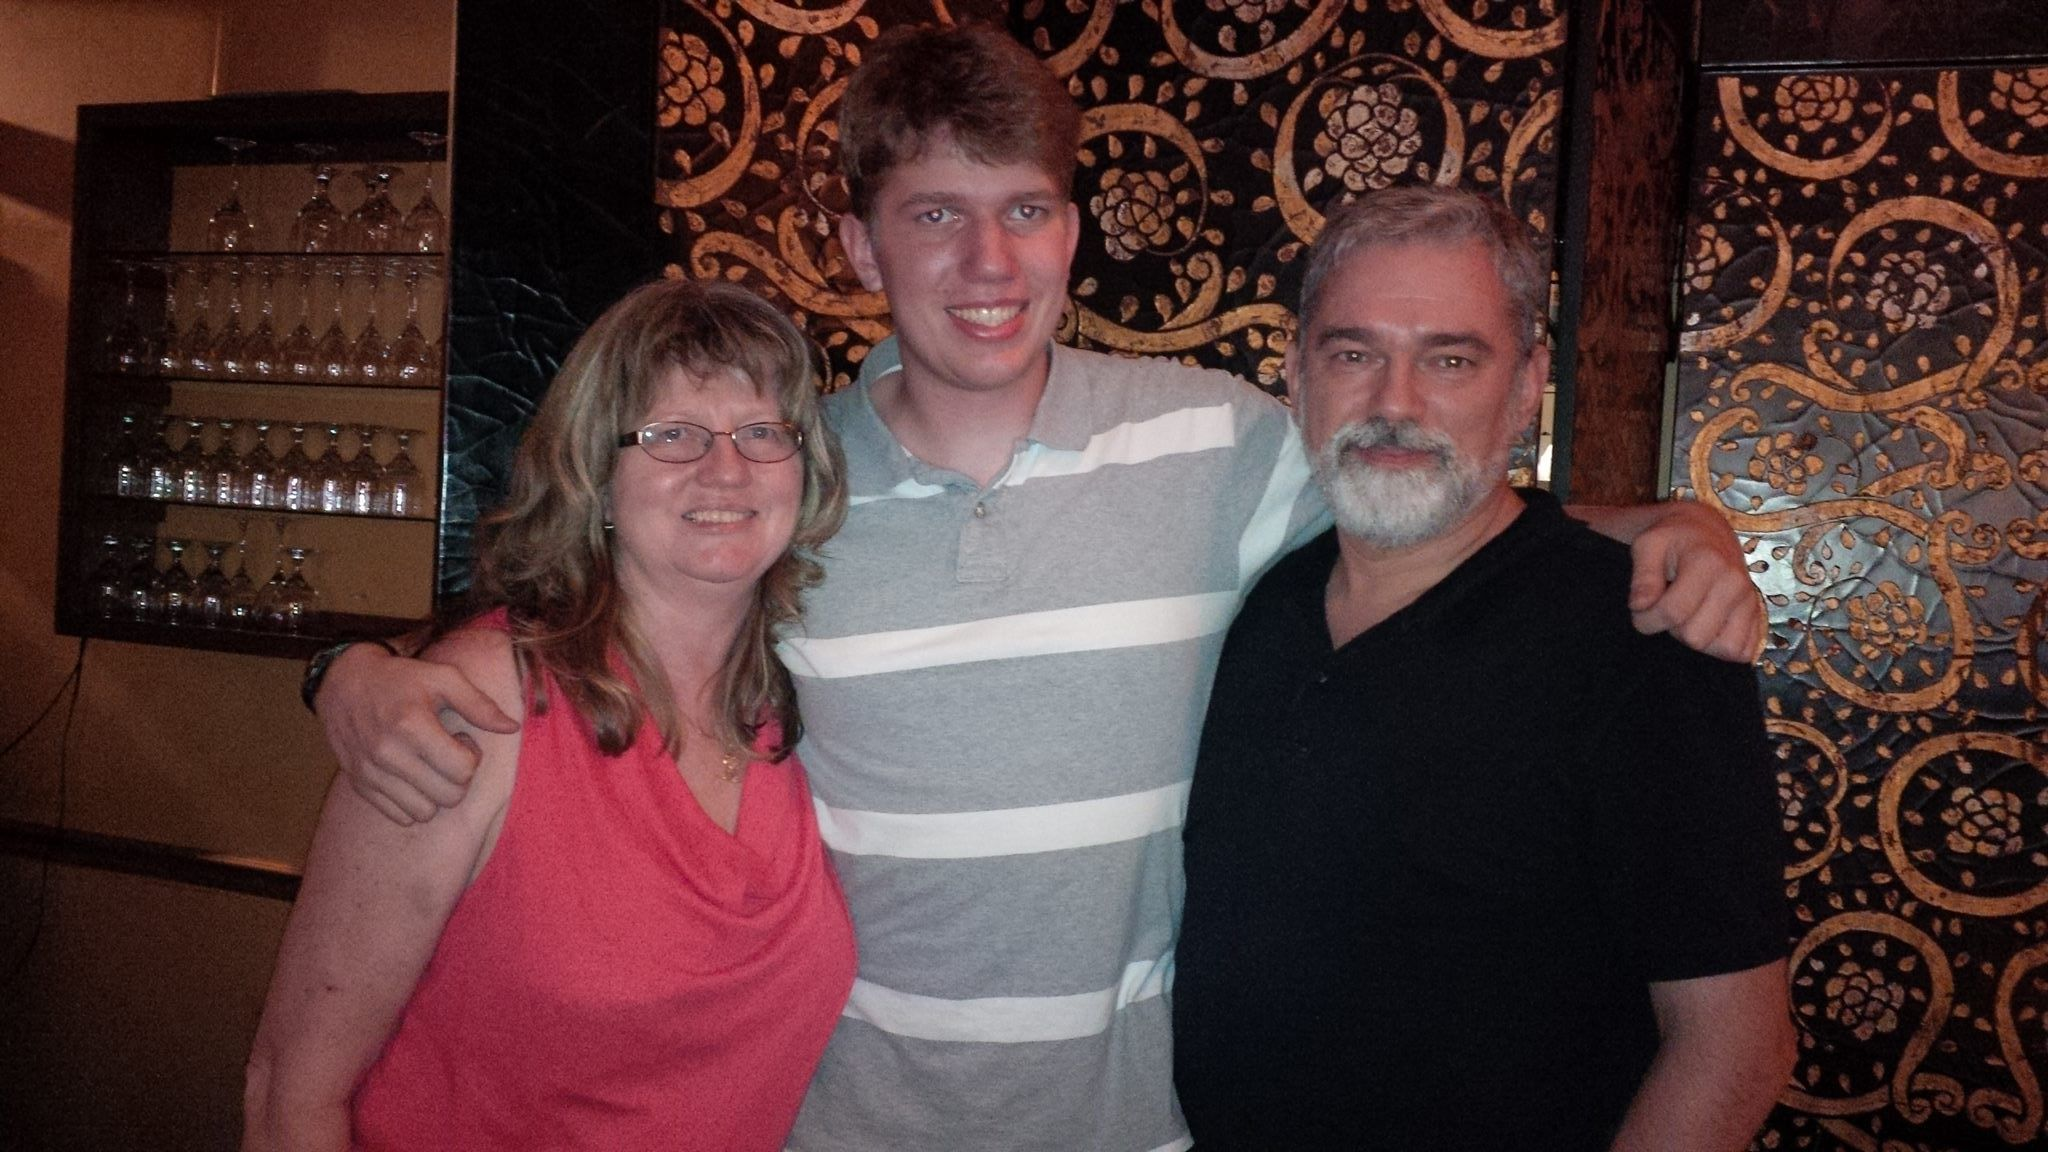
\includegraphics[height=6cm]{../img/family.jpg}
\end{center}
\end{frame}


%
% Group + Friends
%
\begin{frame}[noframenumbering]{Thanks!}
\begin{center}
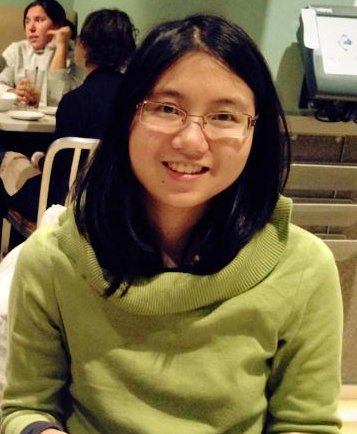
\includegraphics[height=3cm]{../img/sharon.jpg}
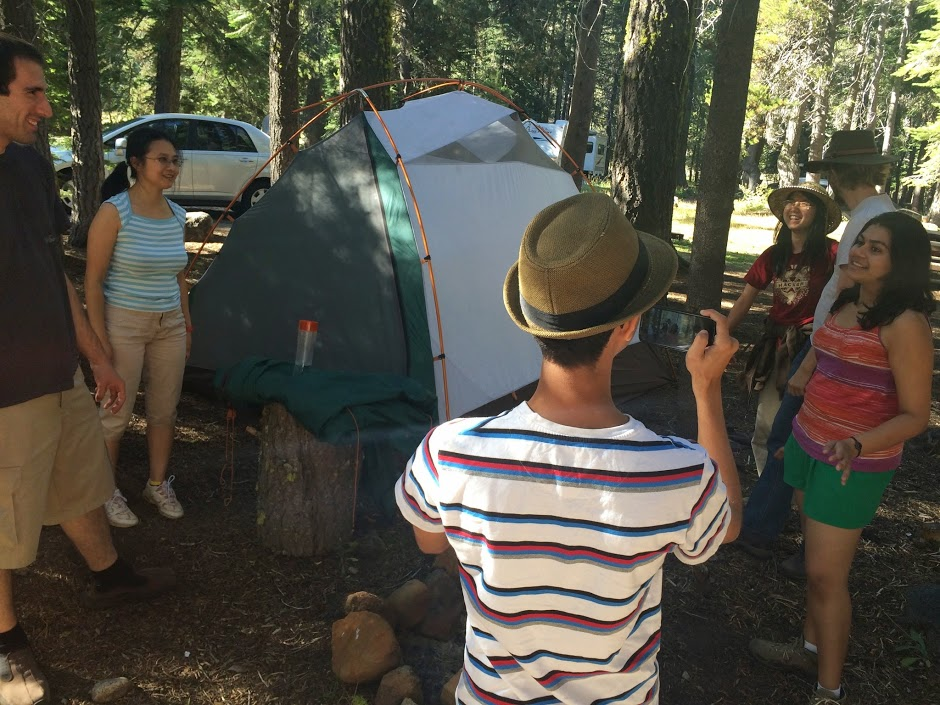
\includegraphics[height=3cm]{../img/friends-1.jpg}
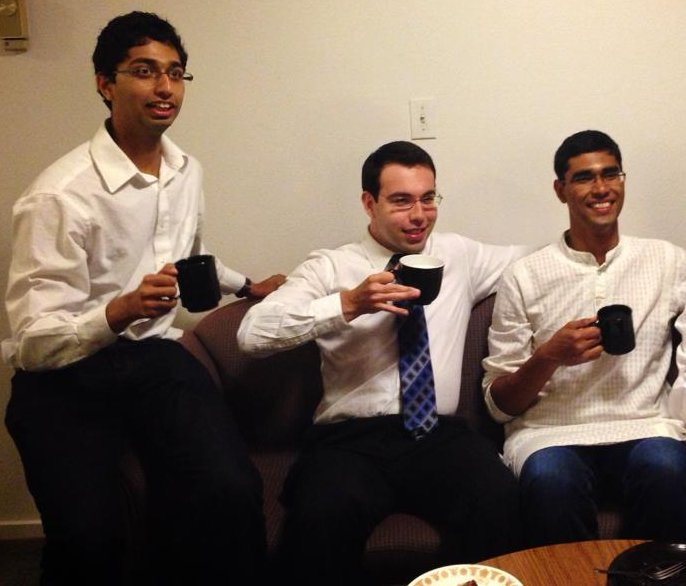
\includegraphics[height=3cm]{../img/friends-2.jpg}
\\
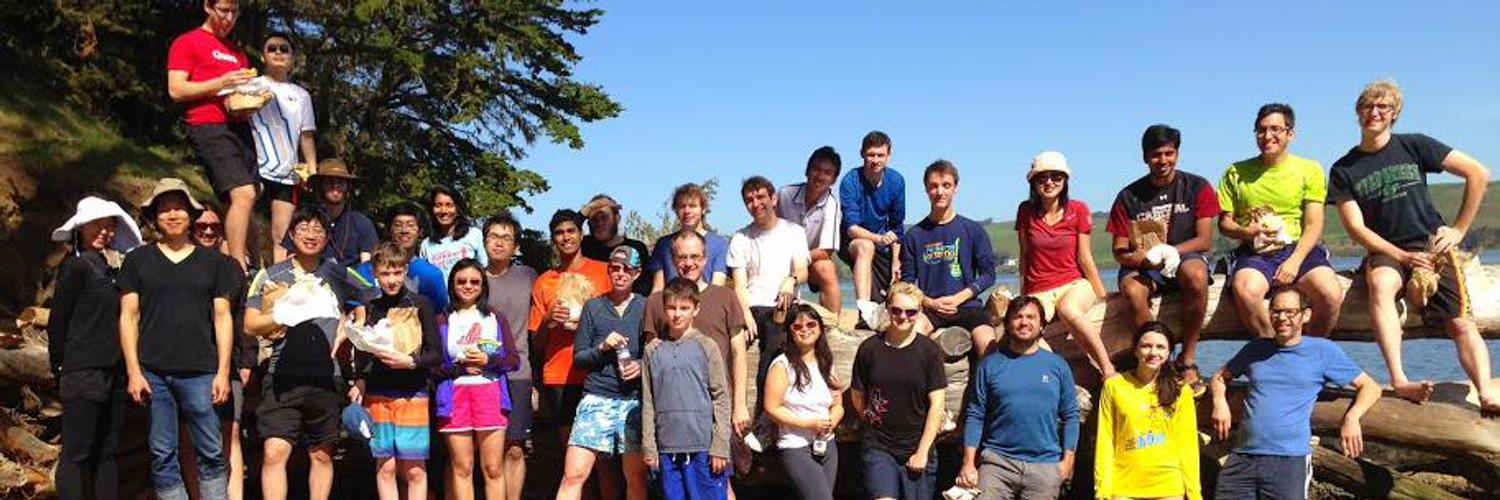
\includegraphics[width=10cm]{../img/nlp-group.jpg}
\end{center}
\end{frame}

%
% Questions
%
\begin{frame}[noframenumbering]{Questions?}
\begin{center}
\includegraphics[height=6cm]{../img/xkcd-defense.png}
\end{center}
\end{frame}
